%%% BEGIN UNIT
\wbunit{Fracciones en la recta y en colecciones}{Vas a ver las fracciones en la recta numérica y cuando son parte de un grupo de objetos.}

\section{Fracciones unitarias}

Imagina que compartes una barra de chocolate con tus amigos. Si la partes en partes iguales, cada parte es una fracción de la barra completa.

Primero lo vemos concreto: una barra real partida en 4 trozos iguales. Luego lo dibujamos: una barra pintada. Al final lo escribimos con números: $\frac{1}{4}$.

Cuando tomas \textbf{una sola} de esas partes iguales, tienes una fracción unitaria.

\begin{wbidea}[Fracción unitaria]
Una \textbf{fracción unitaria} es $\frac{1}{b}$. Significa 1 parte de $b$ partes iguales en que se dividió el todo.

El denominador $b$ dice en cuántas partes iguales se dividió el todo. El numerador $1$ dice que tomas una parte.

Ejemplo: $\frac{1}{4}$ es una de cuatro partes iguales.
\end{wbidea}

Mira cómo se ve $\frac{1}{4}$ con diferentes dibujos:

\begin{center}
\wbfracbar[6cm]{1}{4} \hspace{1cm} \wbfraccircle{1}{4}
\end{center}

Las dos figuras están divididas en 4 partes iguales y 1 parte está pintada. Las dos muestran $\frac{1}{4}$.

Si juntas varias fracciones unitarias iguales, formas otras fracciones. Por ejemplo, $\frac{3}{4}$ son tres copias de $\frac{1}{4}$:

\begin{center}
\wbfracbar[6cm]{1}{4} \hspace{0.3cm} + \hspace{0.3cm} \wbfracbar[6cm]{1}{4} \hspace{0.3cm} + \hspace{0.3cm} \wbfracbar[6cm]{1}{4} \hspace{0.3cm} = \hspace{0.3cm} \wbfracbar[6cm]{3}{4}
\end{center}
\[ \frac{1}{4} + \frac{1}{4} + \frac{1}{4} = \frac{3}{4} \]

\begin{wbexample}[Escribir la fracción unitaria de una barra]
Una tira de papel está dividida en 3 partes iguales. Solo 1 parte está pintada de azul. ¿Qué fracción está pintada?

\begin{center}
\wbfracbar[8cm]{1}{3}
\end{center}

\textbf{Solución paso a paso:}
\begin{enumerate}
\item Cuenta en cuántas partes iguales está dividida la tira. Son $3$ partes.
\item Ese número va abajo: denominador $3$.
\item Cuenta cuántas partes están pintadas. Es $1$ parte.
\item Ese número va arriba: numerador $1$.
\item La fracción es $\frac{1}{3}$.
\end{enumerate}
\end{wbexample}

\begin{wbexample}[Formar una fracción con fracciones unitarias]
¿Cuántas copias de $\frac{1}{6}$ necesitas para formar $\frac{5}{6}$? Dibuja y escribe.

\textbf{Solución paso a paso:}
\begin{enumerate}
\item $\frac{1}{6}$ es una parte de seis iguales.
\begin{center}
\wbfracbar[6cm]{1}{6}
\end{center}
\item Para tener $\frac{5}{6}$ necesitas 5 de esas partes.
\begin{center}
\wbfracbar[6cm]{5}{6}
\end{center}
\item Cuenta: $\frac{1}{6} + \frac{1}{6} + \frac{1}{6} + \frac{1}{6} + \frac{1}{6} = \frac{5}{6}$.
\item Respuesta: necesitas \textbf{5 copias} de $\frac{1}{6}$.
\end{enumerate}
\end{wbexample}

\begin{wbtip}[¡Ojo con las partes iguales!]
Para que sea una fracción, todas las partes deben ser del mismo tamaño. Si las partes no son iguales, no puedes escribir $\frac{1}{b}$.
\begin{center}
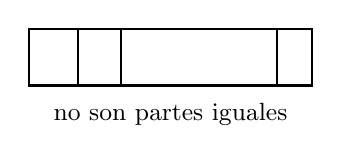
\begin{tikzpicture}[scale=0.9]
\draw[thick] (0,0) rectangle (4,0.8);
\draw[thick] (0.7,0) -- (0.7,0.8);
\draw[thick] (1.3,0) -- (1.3,0.8);
\draw[thick] (3.5,0) -- (3.5,0.8);
\node at (2,-0.4) {\small no son partes iguales};
\end{tikzpicture}
\hspace{1cm}
\begin{tikzpicture}[scale=0.9]
\draw[thick] (0,0) rectangle (4,0.8);
\draw[thick] (1,0) -- (1,0.8);
\draw[thick] (2,0) -- (2,0.8);
\draw[thick] (3,0) -- (3,0.8);
\fill[wbaccent!30] (0,0) rectangle (1,0.8);
\node at (2,-0.4) {\small sí son partes iguales: $\frac{1}{4}$};
\end{tikzpicture}
\end{center}
\end{wbtip}

\begin{wbpractice}
\begin{enumerate}
\item Observa el círculo. Está dividido en 4 partes iguales y 1 parte está pintada. ¿Qué fracción está pintada?
\begin{center}
\wbfraccircle{1}{4}
\end{center}
Escribe la fracción: \wbfracbox
\wblines{1}

\item Observa la barra. ¿Qué fracción unitaria está pintada?
\begin{center}
\wbfracbar[8cm]{1}{5}
\end{center}
Escribe la fracción: \wbfracbox
\wblines{1}

\item Pinta la barra para mostrar $\frac{1}{3}$. La barra ya está dividida en 3 partes iguales.
\begin{center}
\wbfracbar[8cm]{0}{3}
\end{center}
\wbbox[1.5cm]
\wblines{1}

\item Pinta el círculo para mostrar $\frac{1}{6}$. El círculo ya está dividido en 6 partes iguales.
\begin{center}
\wbfraccircle{0}{6}
\end{center}
\wbbox[1.5cm]
\wblines{1}

\item Completa: $\frac{3}{5}$ son \wbblank\ copias de $\frac{1}{5}$. Dibuja las barras si te ayuda.
\begin{center}
\wbfracbar[6cm]{1}{5} \hspace{0.5cm} \wbfracbar[6cm]{3}{5}
\end{center}
\wblines{2}

\item Ana corta una pizza en 8 rebanadas iguales y toma 1 rebanada. ¿Qué fracción de la pizza tomó Ana? Explica con un dibujo.
\wbbox[2cm]
Escribe la fracción: \wbfracbox
\wblines{2}

\item ¿Cuál es más grande, $\frac{1}{2}$ o $\frac{1}{8}$? Usa las barras para explicar tu respuesta con palabras o dibujo.
\begin{center}
\wbfracbar[6cm]{1}{2} \hspace{0.5cm} \wbfracbar[6cm]{1}{8}
\end{center}
\wblines{3}
\end{enumerate}
\end{wbpractice}

\section{La recta numérica del 0 al 1}

La recta numérica también nos ayuda a ver fracciones. Imagina que caminas del $0$ al $1$. Si divides ese camino en partes iguales, cada paso es una fracción unitaria.

\begin{wbidea}[Fracciones en la recta del 0 al 1]
Para mostrar fracciones entre $0$ y $1$:
\begin{enumerate}
\item Divide el segmento de $0$ a $1$ en $b$ partes iguales.
\item Cada parte mide $\frac{1}{b}$.
\item Para llegar a $\frac{a}{b}$, avanza $a$ pasos de $\frac{1}{b}$ desde el $0$.
\end{enumerate}
\end{wbidea}

Ejemplo con cuartos. Dividimos de $0$ a $1$ en 4 partes iguales. Cada salto es $\frac{1}{4}$.

\begin{center}
\wbnumberline[10cm]{4}{1}{1,2,3}
\end{center}

El primer punto después del $0$ es $\frac{1}{4}$, el siguiente es $\frac{2}{4}$, luego $\frac{3}{4}$ y al final $1$ que es $\frac{4}{4}$.

\begin{wbexample}[Ubicar $\frac{3}{4}$ en la recta]
Ubica $\frac{3}{4}$ en la recta del $0$ al $1$ dividida en cuartos.

\begin{center}
\wbnumberline[10cm]{4}{1}{}
\end{center}

\textbf{Solución paso a paso:}
\begin{enumerate}
\item Verifica que de $0$ a $1$ hay $4$ partes iguales. Cada parte es $\frac{1}{4}$.
\item Empieza en $0$ y cuenta 3 pasos de $\frac{1}{4}$: $1$, $2$, $3$.
\item Marca el tercer punto y escribe $\frac{3}{4}$.
\end{enumerate}
\begin{center}
\wbnumberline[10cm]{4}{1}{3}
\end{center}
\end{wbexample}

\begin{wbexample}[Leer una fracción en la recta]
¿Qué fracción marca el punto rojo en esta recta?

\begin{center}
\wbnumberline[10cm]{3}{1}{2}
\end{center}

\textbf{Solución paso a paso:}
\begin{enumerate}
\item Cuenta en cuántas partes iguales está dividido de $0$ a $1$. Son $3$ partes, entonces cada parte es $\frac{1}{3}$.
\item Cuenta cuántos pasos hay desde $0$ hasta el punto. Hay $2$ pasos.
\item El punto es $\frac{2}{3}$.
\end{enumerate}
\end{wbexample}

\begin{wbtip}[Cuenta desde el 0]
En la recta, siempre empieza a contar desde el $0$, no desde el $1$. El primer salto después del $0$ es $\frac{1}{b}$, no $\frac{0}{b}$.
\begin{center}
\begin{tikzpicture}[scale=1]
\draw[thick,->] (0,0) -- (6,0);
\foreach \x in {0,1.5,3,4.5,6} \draw[thick] (\x,0.15) -- (\x,-0.15);
\node at (0,-0.4) {$0$};
\node at (1.5,-0.4) {$\frac{1}{4}$};
\node at (3,-0.4) {$\frac{2}{4}$};
\node at (4.5,-0.4) {$\frac{3}{4}$};
\node at (6,-0.4) {$1$};
\draw[wbaccent,thick,->] (0,0.3) -- (1.5,0.3);
\node at (0.75,0.6) {\small 1 paso};
\end{tikzpicture}
\end{center}
\end{wbtip}

\begin{wbpractice}
\begin{enumerate}
\item Escribe la fracción que marca cada punto en esta recta de mitades.
\begin{center}
\wbnumberline[10cm]{2}{1}{1}
\end{center}
El punto marca \wbfracbox
\wblines{1}

\item Escribe la fracción que marca el punto rojo en esta recta de sextos.
\begin{center}
\wbnumberline[10cm]{6}{1}{4}
\end{center}
El punto marca \wbfracbox
\wblines{1}

\item Ubica $\frac{1}{8}$ en la recta. La recta está dividida en 8 partes iguales. Marca el punto con una X.
\begin{center}
\wbnumberline[10cm]{8}{1}{}
\end{center}
\wbbox[1cm]
\wblines{1}

\item Ubica $\frac{5}{6}$ en la recta. La recta está dividida en 6 partes iguales. Marca el punto con una X.
\begin{center}
\wbnumberline[10cm]{6}{1}{}
\end{center}
\wbbox[1cm]
\wblines{1}

\item Completa los números que faltan en esta recta de tercios.
\begin{center}
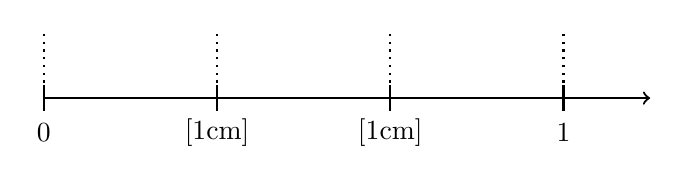
\begin{tikzpicture}[scale=1.1]
\draw[thick,->] (0,0) -- (7,0);
\foreach \x in {0,2,4,6} \draw[thick] (\x,0.15) -- (\x,-0.15);
\foreach \x in {0,2,4,6} \draw[thick,dotted] (\x,0) -- (\x,0.8);
\node at (0,-0.4) {$0$};
\node at (2,-0.4) {\wbblank[1cm]};
\node at (4,-0.4) {\wbblank[1cm]};
\node at (6,-0.4) {$1$};
\end{tikzpicture}
\end{center}
\wblines{2}

\item Una rana salta $\frac{1}{4}$ cada vez. Empieza en $0$. ¿En qué fracción cae después de 3 saltos? Marca en la recta.
\begin{center}
\wbnumberline[10cm]{4}{1}{}
\end{center}
Respuesta: \wbfracbox
\wblines{2}

\item En la recta de cuartos, ¿qué punto está más cerca del $1$: $\frac{1}{4}$ o $\frac{3}{4}$? Explica cómo lo sabes mirando la recta.
\begin{center}
\wbnumberline[10cm]{4}{1}{1,3}
\end{center}
\wblines{3}
\end{enumerate}
\end{wbpractice}

\section{Fracciones de una colección}

A veces la fracción no es parte de una sola cosa, sino parte de un grupo de objetos. Por ejemplo, $\frac{1}{2}$ de 6 pelotas.

Para hallarlo, repartes los objetos en grupos iguales.

\begin{wbidea}[Fracción de una colección]
Para hallar $\frac{1}{b}$ de una colección de objetos:
\begin{enumerate}
\item Divide todos los objetos en $b$ grupos iguales.
\item Cada grupo es $\frac{1}{b}$ de la colección.
\item Cuenta cuántos objetos hay en un grupo.
\end{enumerate}
\end{wbidea}

Ejemplo: $\frac{1}{2}$ de 6 pelotas.

\begin{center}
\begin{tikzpicture}[scale=0.8]
\foreach \x in {0,1,2} \fill[wbprimary] (\x*0.7,0.6) circle (0.22);
\foreach \x in {0,1,2} \fill[wbprimary] (\x*0.7,-0.6) circle (0.22);
\draw[wbaccent,thick,dashed] (-0.4,1.1) rectangle (2.5,-0.1);
\draw[wbaccent,thick,dashed] (-0.4,-0.1) rectangle (2.5,-1.1);
\node at (1,1.4) {\small grupo 1: 3};
\node at (1,-1.4) {\small grupo 2: 3};
\end{tikzpicture}
\end{center}

Dividimos 6 pelotas en 2 grupos iguales. Cada grupo tiene 3 pelotas. Entonces $\frac{1}{2}$ de 6 es $3$.

También puedes usar una barra:

\begin{center}
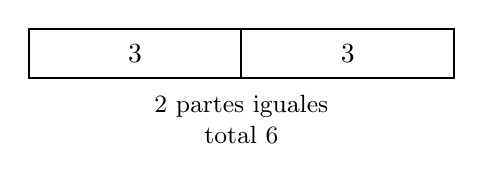
\begin{tikzpicture}[scale=0.9]
\draw[thick] (0,0) rectangle (6,0.7);
\draw[thick] (3,0) -- (3,0.7);
\node at (1.5,0.35) {3};
\node at (4.5,0.35) {3};
\node at (3,-0.4) {\small 2 partes iguales};
\node at (3,-0.8) {\small total 6};
\end{tikzpicture}
\end{center}

\begin{wbexample}[Hallar $\frac{1}{3}$ de 12 canicas]
Hay 12 canicas. ¿Cuánto es $\frac{1}{3}$ de 12?

\textbf{Solución paso a paso:}
\begin{enumerate}
\item Divide 12 canicas en 3 grupos iguales.
\begin{center}
\begin{tikzpicture}[scale=0.7]
\foreach \x in {0,1,2,3} \fill[wbprimary] (\x*0.6,0.8) circle (0.2);
\foreach \x in {0,1,2,3} \fill[wbsecondary] (\x*0.6,0) circle (0.2);
\foreach \x in {0,1,2,3} \fill[wbaccent] (\x*0.6,-0.8) circle (0.2);
\draw[thick,dashed,rounded corners] (-0.4,1.2) rectangle (2.8,0.4);
\draw[thick,dashed,rounded corners] (-0.4,0.4) rectangle (2.8,-0.4);
\draw[thick,dashed,rounded corners] (-0.4,-0.4) rectangle (2.8,-1.2);
\node at (1.2,1.6) {\small grupo 1: 4};
\node at (1.2,-1.6) {\small grupo 3: 4};
\node at (4,0) {\small grupo 2: 4};
\end{tikzpicture}
\end{center}
\item Reparte una por una: 12 $\div$ 3 = 4.
\item Cada grupo tiene 4 canicas.
\item Respuesta: $\frac{1}{3}$ de 12 es \textbf{4 canicas}.
\end{enumerate}
\end{wbexample}

\begin{wbexample}[Hallar $\frac{1}{4}$ de 8 lápices]
Hay 8 lápices. ¿Cuánto es $\frac{1}{4}$ de 8?

\textbf{Solución paso a paso:}
\begin{enumerate}
\item Divide 8 lápices en 4 grupos iguales.
\begin{center}
\begin{tikzpicture}[scale=0.8]
\foreach \i in {0,1} \fill[wbprimary] (\i*0.6,0) circle (0.18);
\foreach \i in {0,1} \fill[wbsecondary] (2+\i*0.6,0) circle (0.18);
\foreach \i in {0,1} \fill[wbaccent] (4+\i*0.6,0) circle (0.18);
\foreach \i in {0,1} \fill[wbprimary!60!wbsecondary] (6+\i*0.6,0) circle (0.18);
\draw[dashed] (-0.3,-0.4) rectangle (1.1,0.4);
\draw[dashed] (1.7,-0.4) rectangle (3.1,0.4);
\draw[dashed] (3.7,-0.4) rectangle (5.1,0.4);
\draw[dashed] (5.7,-0.4) rectangle (7.1,0.4);
\node at (0.4,-0.8) {\small 2};
\node at (2.4,-0.8) {\small 2};
\node at (4.4,-0.8) {\small 2};
\node at (6.4,-0.8) {\small 2};
\end{tikzpicture}
\end{center}
\item 8 $\div$ 4 = 2.
\item Cada grupo tiene 2 lápices.
\item Respuesta: $\frac{1}{4}$ de 8 es \textbf{2 lápices}.
\end{enumerate}
\end{wbexample}

\begin{wbtip}[No confundas el número de grupos con el número de objetos]
El denominador te dice cuántos grupos iguales debes hacer, no cuántos objetos hay en cada grupo. Para $\frac{1}{3}$ de 12, haces 3 grupos, no grupos de 3.
\end{wbtip}

\begin{wbpractice}
\begin{enumerate}
\item ¿Cuánto es $\frac{1}{2}$ de 10 estrellas? Divide en 2 grupos iguales.
\begin{center}
\begin{tikzpicture}[scale=0.7]
\foreach \x in {0,1,2,3,4} \foreach \y in {0,1} \fill[wbprimary] (\x*0.7,\y*0.7) circle (0.18);
\end{tikzpicture}
\end{center}
\wbbox[1.5cm]
Respuesta: \wbblank\ estrellas
\wblines{1}

\item ¿Cuánto es $\frac{1}{4}$ de 12 galletas? Dibuja 4 grupos iguales.
\begin{center}
\begin{tikzpicture}[scale=0.7]
\foreach \x in {0,1,2,3} \foreach \y in {0,1,2} \fill[wbaccent] (\x*0.7,\y*0.7) circle (0.18);
\end{tikzpicture}
\end{center}
\wbbox[1.5cm]
Respuesta: \wbblank\ galletas
\wblines{1}

\item ¿Cuánto es $\frac{1}{3}$ de 9 carritos? 
\begin{center}
\begin{tikzpicture}[scale=0.7]
\foreach \x in {0,1,2,3,4,5,6,7,8} \fill[wbsecondary] (\x*0.6,0) circle (0.2);
\end{tikzpicture}
\end{center}
Respuesta: \wbblank\ carritos
\wblines{2}

\item Hay 16 colores. $\frac{1}{8}$ de los colores son rojos. ¿Cuántos colores son rojos?
\wbbox[1.5cm]
Respuesta: \wbblank\ colores
\wblines{2}

\item En una caja hay 15 pelotas. $\frac{1}{5}$ son azules. ¿Cuántas pelotas son azules? Usa la barra si te ayuda.
\begin{center}
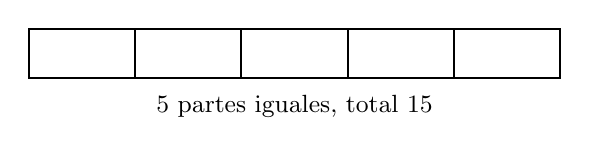
\begin{tikzpicture}[scale=0.9]
\draw[thick] (0,0) rectangle (7.5,0.7);
\foreach \x in {1.5,3,4.5,6} \draw[thick] (\x,0) -- (\x,0.7);
\node at (3.75,-0.4) {\small 5 partes iguales, total 15};
\end{tikzpicture}
\end{center}
Respuesta: \wbblank\ pelotas
\wblines{2}

\item Problema: Sofía tiene 18 canicas y regala $\frac{1}{3}$ a su hermano. ¿Cuántas canicas regala?
\wbbox[2cm]
Respuesta: \wbblank\ canicas
\wblines{2}

\item Si $\frac{1}{4}$ de una colección es 5 lápices, ¿cuántos lápices hay en total? Pista: hay 4 grupos iguales y uno tiene 5.
\wbbox[2cm]
Respuesta: \wbblank\ lápices en total
\wblines{3}
\end{enumerate}
\end{wbpractice}

\begin{wbreview}
\begin{enumerate}
\item Escribe la fracción unitaria que muestra la parte pintada.
\begin{center}
\wbfracbar[7cm]{1}{6}
\end{center}
\wbfracbox
\wblines{1}

\item Pinta $\frac{1}{8}$ de la barra.
\begin{center}
\wbfracbar[8cm]{0}{8}
\end{center}
\wbbox[1cm]
\wblines{1}

\item ¿Cuántas copias de $\frac{1}{4}$ forman $\frac{3}{4}$? \wbblank\ copias
\wblines{1}

\item Escribe la fracción que marca el punto en la recta.
\begin{center}
\wbnumberline[10cm]{4}{1}{2}
\end{center}
\wbfracbox
\wblines{1}

\item Ubica $\frac{7}{8}$ en la recta de octavos. Marca con una X.
\begin{center}
\wbnumberline[10cm]{8}{1}{}
\end{center}
\wbbox[1cm]
\wblines{1}

\item ¿Cuánto es $\frac{1}{3}$ de 15 manzanas? \wbblank\ manzanas
\wblines{2}

\item Hay 20 libros. $\frac{1}{4}$ son de cuentos. ¿Cuántos son de cuentos? \wbblank\ libros
\wblines{2}

\item Problema: En un salón hay 24 estudiantes. $\frac{1}{6}$ llevan gorra. ¿Cuántos llevan gorra?
\wbbox[2cm]
\wblines{2}

\item Explica con tus palabras qué significa $\frac{1}{5}$ usando un dibujo o un ejemplo de tu vida.
\wbbox[2.5cm]
\wblines{3}
\end{enumerate}
\end{wbreview}
%%% END UNIT
%%% BEGIN ANSWERS
\wbanswers{\wbLPractice\ 2.1}
\begin{enumerate}
\item $\frac{1}{4}$
\item $\frac{1}{5}$
\item Barra con 1 de 3 partes pintada. Cualquier parte pintada vale si es una sola.
\item Círculo con 1 de 6 partes pintada.
\item 3 copias. $\frac{1}{5}+\frac{1}{5}+\frac{1}{5}=\frac{3}{5}$.
\item $\frac{1}{8}$. Dibujo: círculo o barra dividido en 8 partes iguales con 1 parte pintada.
\item $\frac{1}{2}$ es más grande. En la barra se ve que $\frac{1}{2}$ ocupa más espacio que $\frac{1}{8}$. Con el mismo todo, entre menos partes, más grande es cada parte.
\end{enumerate}

\wbanswers{\wbLPractice\ 2.2}
\begin{enumerate}
\item $\frac{1}{2}$
\item $\frac{4}{6}$ (o $\frac{2}{3}$ si simplifica, pero se espera $\frac{4}{6}$ en sextos)
\item Punto marcado en la primera marca después del 0. Es $\frac{1}{8}$.
\item Punto marcado en la quinta marca después del 0. Es $\frac{5}{6}$.
\item De izquierda a derecha: $\frac{1}{3}$, $\frac{2}{3}$. Cada salto es $\frac{1}{3}$.
\item $\frac{3}{4}$. Tres saltos de $\frac{1}{4}$ desde 0.
\item $\frac{3}{4}$ está más cerca del 1. En la recta $\frac{3}{4}$ está a un salto de 1 y $\frac{1}{4}$ está a tres saltos de 1.
\end{enumerate}

\wbanswers{\wbLPractice\ 2.3}
\begin{enumerate}
\item 5 estrellas. 10 $\div$ 2 = 5. Dos grupos de 5.
\item 3 galletas. 12 $\div$ 4 = 3. Cuatro grupos de 3.
\item 3 carritos. 9 $\div$ 3 = 3.
\item 2 colores. 16 $\div$ 8 = 2.
\item 3 pelotas. 15 $\div$ 5 = 3.
\item 6 canicas. 18 $\div$ 3 = 6.
\item 20 lápices. Si un grupo de 4 tiene 5, total $4 \times 5 = 20$.
\end{enumerate}

\wbanswers{\wbLReview}
\begin{enumerate}
\item $\frac{1}{6}$
\item Barra con 1 de 8 partes pintada.
\item 3 copias.
\item $\frac{2}{4}$ (equivale a $\frac{1}{2}$)
\item Punto marcado en la séptima marca después del 0. Es $\frac{7}{8}$.
\item 5 manzanas. 15 $\div$ 3 = 5.
\item 5 libros. 20 $\div$ 4 = 5.
\item 4 estudiantes. 24 $\div$ 6 = 4.
\item Respuesta abierta. Debe decir que $\frac{1}{5}$ es una parte de cinco partes iguales de un todo o de una colección. Dibujo debe mostrar división en 5 partes iguales con 1 parte señalada. Ejemplo válido: una barra, pizza o 5 dulces con 1 tomado.
\end{enumerate}
%%% END ANSWERS